%--------------------------------------------------------------------------------------------------------------------
%------------------------------------------------- Chapter 1 --------------------------------------------------------
\chapter{Introducci{\'o}n}
\pagenumbering{arabic}
La mayor{\'\i}a de las plantas petroqu{\'\i}micas y refiner{\'\i}as poseen sistemas de control para
controlar simult{\'a}neamente cientos de variables del proceso, tales como presiones y temperaturas, por
ejemplo. El rol humano principal en estos sistemas de control altamente automatizados es el de
\textit{supervisi{\'o}n}. Esta actividad supervisora requiere: monitoreo del estado actual de la planta, ajuste
de los par{\'a}metros de control, realizar actividades planeadas de operaci{\'o}n y detectar, diagnosticar,
compensar y corregir situaciones anormales.

El incremento de la demanda de alta eficiencia y operaci{\'o}n en estas industrias han derivado en un incremento
muy importante en la sofisticaci{\'o}n de los sistemas de control mediante el desarrollo de estrategias de
control y sensores avanzados. De todas formas estos avances no han eliminado el problema de la presencia de
situaciones anormales.

Una paradoja persistente en el dominio del control supervisor es que a medida que las tecnolog{\'\i}as de
automaci{\'o}n incrementan su complejidad y sofisticaci{\'o}n, los operarios profesionales deben tomar decisiones
cada vez mas complejas para el manejo de situaciones anormales (MSA).

\section{Manejo de situaciones anormales (MSA)}
De forma general una situaci{\'o}n anormal (SA) puede definirse como: \textit{una perturbaci{\'o}n o una serie de
perturbaciones que causan la desviaci{\'o}n de la planta de su punto operativo normal}. La naturaleza de la SA
podr{\'a} ser m{\'\i}nima o catastr{\'o}fica dependiendo de su entorno. Ser{\'a} tarea del equipo de operaciones identificar
la causa de la situaci{\'o}n y ejecutar acciones correctivas o compensatorias de una manera r{\'a}pida y
eficientemente.

Una SA puede generar una reducci{\'o}n en la producci{\'o}n, p{\'e}rdidas en la calidad del producto, da{\~n}os en equipos y
a{\'u}n mas serias poner en riesgo la integridad de las personas. Debido a la naturaleza din{\'a}mica de los
procesos las situaciones anormales se extienden, desarrollan y cambian temporalmente incrementando la
complejidad de los requerimientos de intervenci{\'o}n.

\subsection{Fuentes o causas}\label{sec_fuentes}
Para comprender como abordar tales situaciones, es importante conocer los factores que causan o influyen
sobre las situaciones anormales. En la mayor{\'\i}a de los casos, la SA se presenta como resultado de la
interacci{\'o}n de m{\'u}ltiples fuentes.

Existen tres tipos de causas o fuentes de situaciones anormales
\begin{itemize}
    \item[A.] Factores relacionados con las personas y el entorno de trabajo.
    \item[B.] Factores relacionados con los equipos.
    \item[C.] Factores relacionados con el proceso.
\end{itemize}
una cuarta fuente podr{\'\i}a ser los antecedentes ambientales f{\'\i}sicos (rel{\'a}mpagos, terremotos, tormentas) que no
ser{\'a}n considerados aqu{\'\i} debido a su ocurrencia infrecuente y su generalmente rol obvio como causa ra{\'\i}z.

Las tres fuentes enumeradas anteriormente han sido identificadas de los reportes de incidentes de compa{\~n}{\'\i}as
miembros del consorcio de manejo de situaciones anormales (abnormal situation management consortium ,
\cite{ASM}\textcolor{myblue}{\circledR}) en el per{\'\i}odo 1992--1993. De todos los reportes de incidentes solo
han sido considerados los que tuvieron un impacto sobre la operaci{\'o}n del proceso. Los porcentajes promedio
para cada tipo de fuente se encuentran representados en la Fig. \ref{f0_1}.
%------------------------------------------------------------------------------------------
\begin{figure}[t]
  \centering
  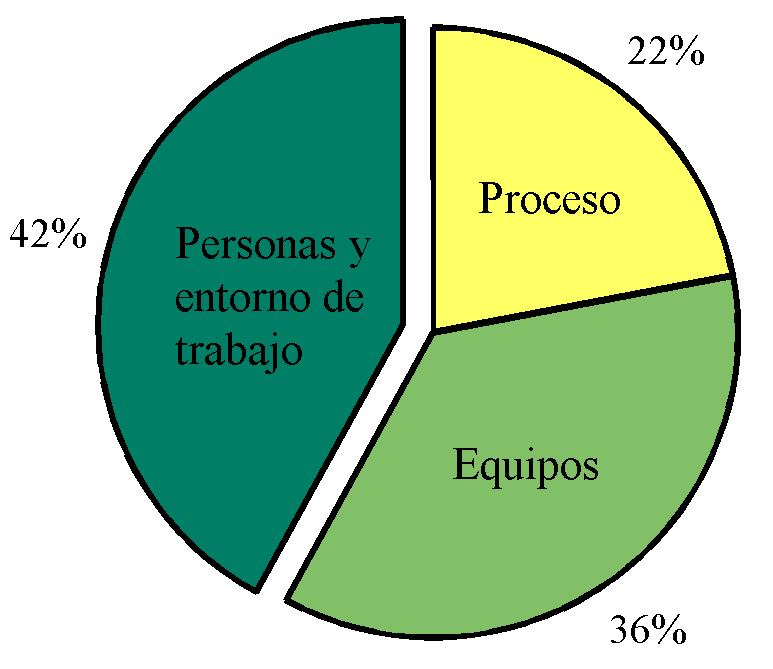
\includegraphics[width=7cm,height=6.2cm]{Ch0/f0_1}\\
  \caption{Porcentajes de fuentes de situaciones anormales (\cite{ASM}\textcolor{myblue}{\circledR})}\label{f0_1}
\end{figure}
%------------------------------------------------------------------------------------------

Los datos provenientes de los reportes de incidentes deben ser analizados con cuidado, ya que podemos
encontrar informaci{\'o}n polarizada de diferentes formas. Los individuos generalmente rechazan la idea de
identificar a las personas como fuente de un incidente y por otro lado, los datos son recolectados de un
peque{\~n}o n{\'u}mero de sitios reflejando la idiosincrasia de tales lugares.

En la Fig. \ref{f0_2} podemos observar la distribuci{\'o}n de la frecuencia, medida en cantidad de incidentes,
de cada fuente identificada. En el caso de personas y entorno de trabajo la causa que mas contribuye a
situaciones anormales es la no existencia de procedimientos o procedimientos inadecuados. En los factores
vinculados con equipos claramente las fallas mec{\'a}nicas son la fuente con mas contribuci{\'o}n. Finalmente, una
mala operaci{\'o}n del proceso superando los l{\'\i}mites originales de de dise{\~n}o son la causa ra{\'\i}z mas probable
cuando hablamos de factores vinculados al proceso.
%------------------------------------------------------------------------------------------
\begin{figure}[t]
  \centering
  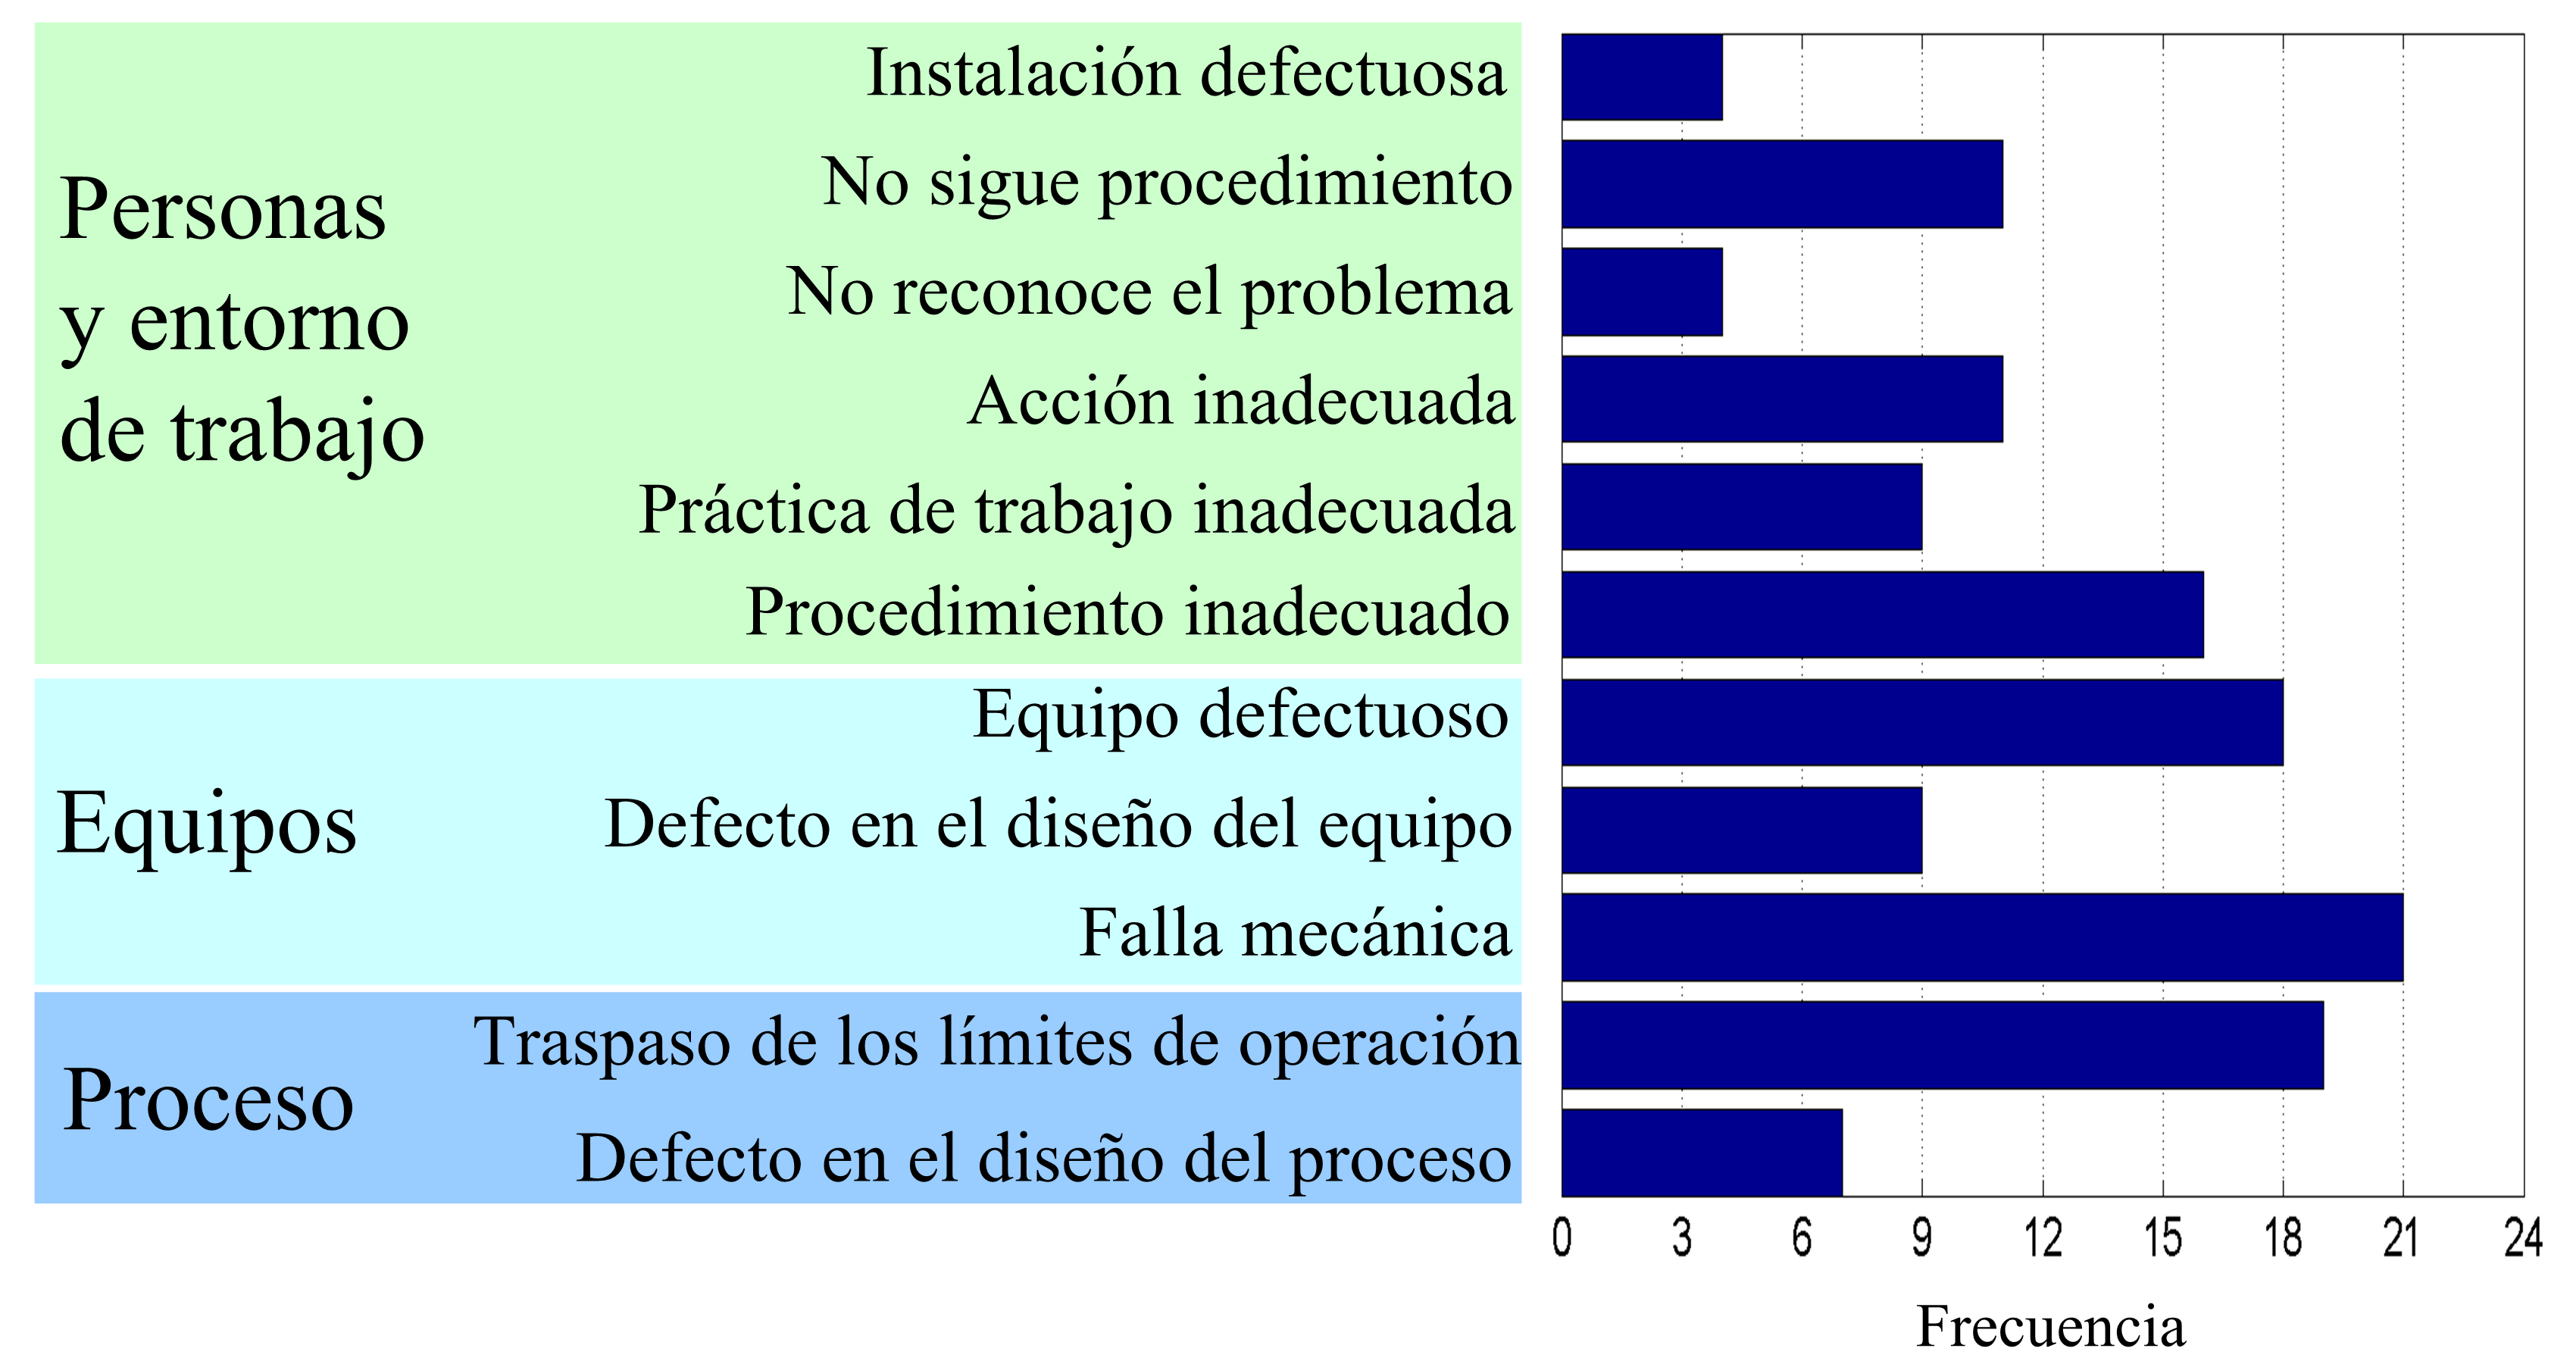
\includegraphics[width=13cm,height=6cm]{Ch0/f0_2}\\
  \caption{Contribuci{\'o}n relativa de cada fuente (\cite{ASM}\textcolor{myblue}{\circledR})}\label{f0_2}
\end{figure}
%------------------------------------------------------------------------------------------

\subsubsection{A. Factores relacionados con las personas y el entorno de trabajo}
Los seres humanos siempre ser{\'a}n una parte del proceso de toma de decisi{\'o}n en las operaciones de planta y por
lo tanto siempre existir{\'a}n oportunidades para errores humanos que contribuyen a las situaciones anormales.
En varios puntos del proceso las personas pueden contribuir a una SA por no responder correctamente con
acciones anticipatorias/compensatorias o por responder con acciones inadecuadas. Las consecuencias de dichos
errores depender{\'a}n de la naturaleza de la SA. Para comprender el rol del personal de planta es importante
clasificar las caracter{\'\i}sticas internas y externas de la toma de decisi{\'o}n que contribuyen a los errores.

Las caracter{\'\i}sticas internas relacionan conceptos como
\begin{itemize}
    \item entrenamiento/habilidad: Los equipos de operaci{\'o}n deben comprender c{\'o}mo trabaja el proceso y
    fundamentalmente c{\'o}mo se utiliza el sistema de control para monitorear la planta. Una carencia de
    entrenamiento contribuye a situaciones anormales;
    \item pr{\'a}ctica/experiencia: Los equipos de operaci{\'o}n deben contar con la experiencia requerida para
    completar sus tareas. La experiencia y la pr{\'a}ctica deben ser distribuidas en todo el personal;
    \item tensi{\'o}n: En el caso de una SA los equipos de operaci{\'o}n deben ser informados pero no abrumados, ya
    que altos niveles de tensi{\'o}n contribuyen a aumentar la probabilidad de errores humanos.
\end{itemize}

Las caracter{\'\i}sticas externas por otro lado relacionan:
\begin{itemize}
    \item estructura de la organizaci{\'o}n: Seg{\'u}n la estructura de organizaci{\'o}n de un equipo de operaciones
    puede tener impacto en la probabilidad de un evento anormal;
    \item comunicaci{\'o}n: Debido a que las operaciones de planta resultan de un esfuerzo coordinado de
    unidades de proceso la habilidad de comunicaci{\'o}n y de informaci{\'o}n es un factor cr{\'\i}tico en la operaci{\'o}n.
    \item procedimientos: La carencia de procedimientos o procedimientos inapropiados pueden contribuir a
    situaciones anormales. Los procedimientos son solamente valiosos si se utilizan.
\end{itemize}

Otras caracter{\'\i}sticas externas pueden ser: pr{\'a}cticas de trabajo, demandas de tareas, entorno, etc.

En conclusi{\'o}n, el personal de planta tiene numerosas cuestiones que monitorear y mantener para que un
proceso cumpla con las condiciones de operabilidad y eficiencia y al mismo tiempo con requisitos de
seguridad.

\subsubsection{B. Factores relacionados con los equipos}
La naturaleza y estado de los equipos de la planta son la mayor causa de situaciones anormales. Una
clasificaci{\'o}n general de los equipos de una planta es: \textit{equipos de proceso} y \textit{equipos de
control}.  El primero hace referencia a equipos tales como bombas, compresores, tanques, reactores,
columnas, etc. y entre las causas de situaciones anormales mas comunes podemos encontrar:
\begin{itemize}
    \item fallas de los equipos: estas refieren a interrupciones en equipos tales como bombas, compresor,
    etc.. Tales aver{\'\i}as pueden causar trastornos significantes en la planta y en un caso extremo podr{\'\i}an
    ocasionar la salida de servicio del proceso. En {\'a}reas cr{\'\i}ticas de la planta pueden utilizarse equipos de
    respaldo;
    \item degradaci{\'o}n del equipo: esta es la situaci{\'o}n anormal m{\'a}s com{\'u}n vinculada a equipos. Este tipo de
    aver{\'\i}a gradual puede resultar en p{\'e}rdidas de producci{\'o}n o de calidad del producto as{\'\i} como tambi{\'e}n en
    una disminuci{\'o}n del rendimiento de control. Son por lo general fallas dif{\'\i}ciles de detectar.
\end{itemize}

Mientras que los equipos de control incluyen sensores, v{\'a}lvulas y controladores. Una gran variedad de
factores relacionados a equipos tales como edad, carga, historial de mantenimiento, etc. pueden impactar en
la naturaleza de la SA. Errores de lectura en un sensor y posicionamiento de una v{\'a}lvula pueden causar una
carga considerable en los equipos de operaci{\'o}n. Decidir sobre el estado del proceso con variables err{\'o}neas
puede traer consecuencias catastr{\'o}ficas.

\begin{itemize}
    \item Fallas en sensores: Existen cuatro modos de fallas en sensores, A) La lectura del sensor esta
    fuera de los l{\'\i}mites del sensor/proceso, B) La lectura del sensor es cambiante a una tasa que est{\'a} fuera
    de los l{\'\i}mites f{\'\i}sicos del proceso o es inconsistente con las caracter{\'\i}sticas del sensor, C) El sensor
    se bloquea dando una medici{\'o}n constante, y D) Sensor con offset (bias), el sensor provee una lectura
    dentro de los l{\'\i}mites f{\'\i}sicos pero es diferente a el valor real. Las mediciones de los sensores
    generalmente se utilizan en lazos autom{\'a}ticos de control, as{\'\i}, un sensor que falla en su lectura puede
    provocar acciones de control err{\'o}neas dejando al proceso en puntos operativos diferentes o incluso
    producir la salida de servicio de la planta.
    \item Fallas en v{\'a}lvulas: De forma similar las v{\'a}lvulas utilizadas para implementar las acciones de
    control pueden sufrir fallas. Un error de posicionamiento de dicha v{\'a}lvula puede causar trastornos
    significantes si los operadores no identifican el problema r{\'a}pidamente.
    \item Fallas en controladores: El advenimiento de los sistemas de control autom{\'a}tico ha complicado la
    tarea de los equipos de operaciones cuando se presenta la necesidad de cambiar a modo de control manual.
    No s{\'o}lo influye la carencia de capacitaci{\'o}n de los equipos de operaciones para controlar manualmente la
    planta sino que tambi{\'e}n se debe tener en cuenta la complejidad del proceso.
\end{itemize}

\subsubsection{C. Factores relacionados con el proceso}
La identificaci{\'o}n de estos factores puede ser un primer paso crucial cuando se pretende aplicar soluciones
para el correcto manejo de situaciones anormales. Los factores inherentes al proceso que afectan la
naturaleza de la SA son:
\begin{itemize}
    \item Tipo de fabricaci{\'o}n: Los procesos qu{\'\i}micos pueden ser clasificados como discontinuos, continuos o
    alguna combinaci{\'o}n de estos. Cada fase de un proceso discontinuo generalmente posee un conjunto
    espec{\'\i}fico de criterios que establecen el {\'e}xito/falla de dicha fase. Se dispone as{\'\i} de procedimientos que
    describen el re-procesamiento de fases que pueden fallar. Cuando una falla ocurre en un proceso
    continuo, la parte del proceso involucrada pierde funcionalidad generando p{\'e}rdidas en la producci{\'o}n o
    la calidad del producto. En un caso extremo, esta puede provocar la salida de servicio de la planta.
    \item Estado de la operaci{\'o}n: El estado operacional de una planta posee una influencia significante en el
    tipo de situaciones anormales y sus consecuencias. Los estados de operaci{\'o}n mayormente encontrados en
    plantas petroqu{\'\i}micas son: \textit{estado estacionario}, \textit{arranque}, \textit{parada} y \textit{transiciones (no incluyen
    arranques/paradas)}. La operaci{\'o}n en estado estacionario es el modo t{\'\i}pico de funcionamiento de procesos
    continuos. El grado de desviaci{\'o}n de dicho estado indica la severidad del evento anormal. El arranque de
    un proceso es una transici{\'o}n infrecuente, en general las condiciones para realizarlo no son conocidas en
    detalle resultando en grandes posibilidades de situaciones anormales. La parada de planta es el tipo de
    transici{\'o}n menos frecuente. Equipos, unidades o plantas pueden ser paradas para mantenimiento preventivo
    o por situaciones de emergencia. Las transiciones de planta desde un punto operativo a otro (procesos
    continuos) generalmente ocurren como consecuencia de cambios en las propiedades de las materias primas,
    cambios en recursos o cambios en la demanda de productos.
    \item Tipo de materiales que son procesados: Las consecuencias de una SA en una planta qu{\'\i}mica tambi{\'e}n
    depende de la naturaleza de los materiales que est{\'a}n siendo procesados. Una clasificaci{\'o}n preliminar de
    materiales manejados puede ser la siguiente: \textit{qu{\'\i}micos peligrosos vs no peligrosos},
    \textit{estado de los qu{\'\i}micos (s{\'o}lido/l{\'\i}quido/gaseoso)} y \textit{sustancias inflamables vs
    no inflamables}. Las acciones correctivas a ser tomadas en caso de situaciones anormales involucrando
    diferentes tipos de materiales pueden ser diferentes, ya sea en t{\'e}rminos de tiempo de respuesta como en
    procedimientos.
    \item Complejidad del proceso: Mientras que es dif{\'\i}cil definir la complejidad de proceso, la mayor{\'\i}a de
    los analistas convienen que cuanto mayor es la complejidad de un proceso, m{\'a}s dif{\'\i}cil es
    manejar una SA. La complejidad de un proceso decrece a medida que los operadores adquieren mayor
    experiencia del proceso. Informaci{\'o}n inadecuada sobre el estado o comportamiento del proceso tambi{\'e}n
    puede ayudar a ver el proceso como uno complejo. Cuando existen m{\'u}ltiples interconexiones entre unidades
    de un proceso, puede resultar sumamente dif{\'\i}cil para los operadores aislar la causa ra{\'\i}z de una SA en
    una unidad en particular.
\end{itemize}

\subsection{Desaf{\'\i}os}
Un aspecto importante del entendimiento del MSA es la interrelaci{\'o}n entre las causas ra{\'\i}z y la intervenci{\'o}n
de los sistemas de planta y el personal. Espec{\'\i}ficamente, la Fig. \ref{f0_3} ilustra la anatom{\'\i}a de un
incidente catastr{\'o}fico.
%------------------------------------------------------------------------------------------
\begin{figure}[t]
  \centering
  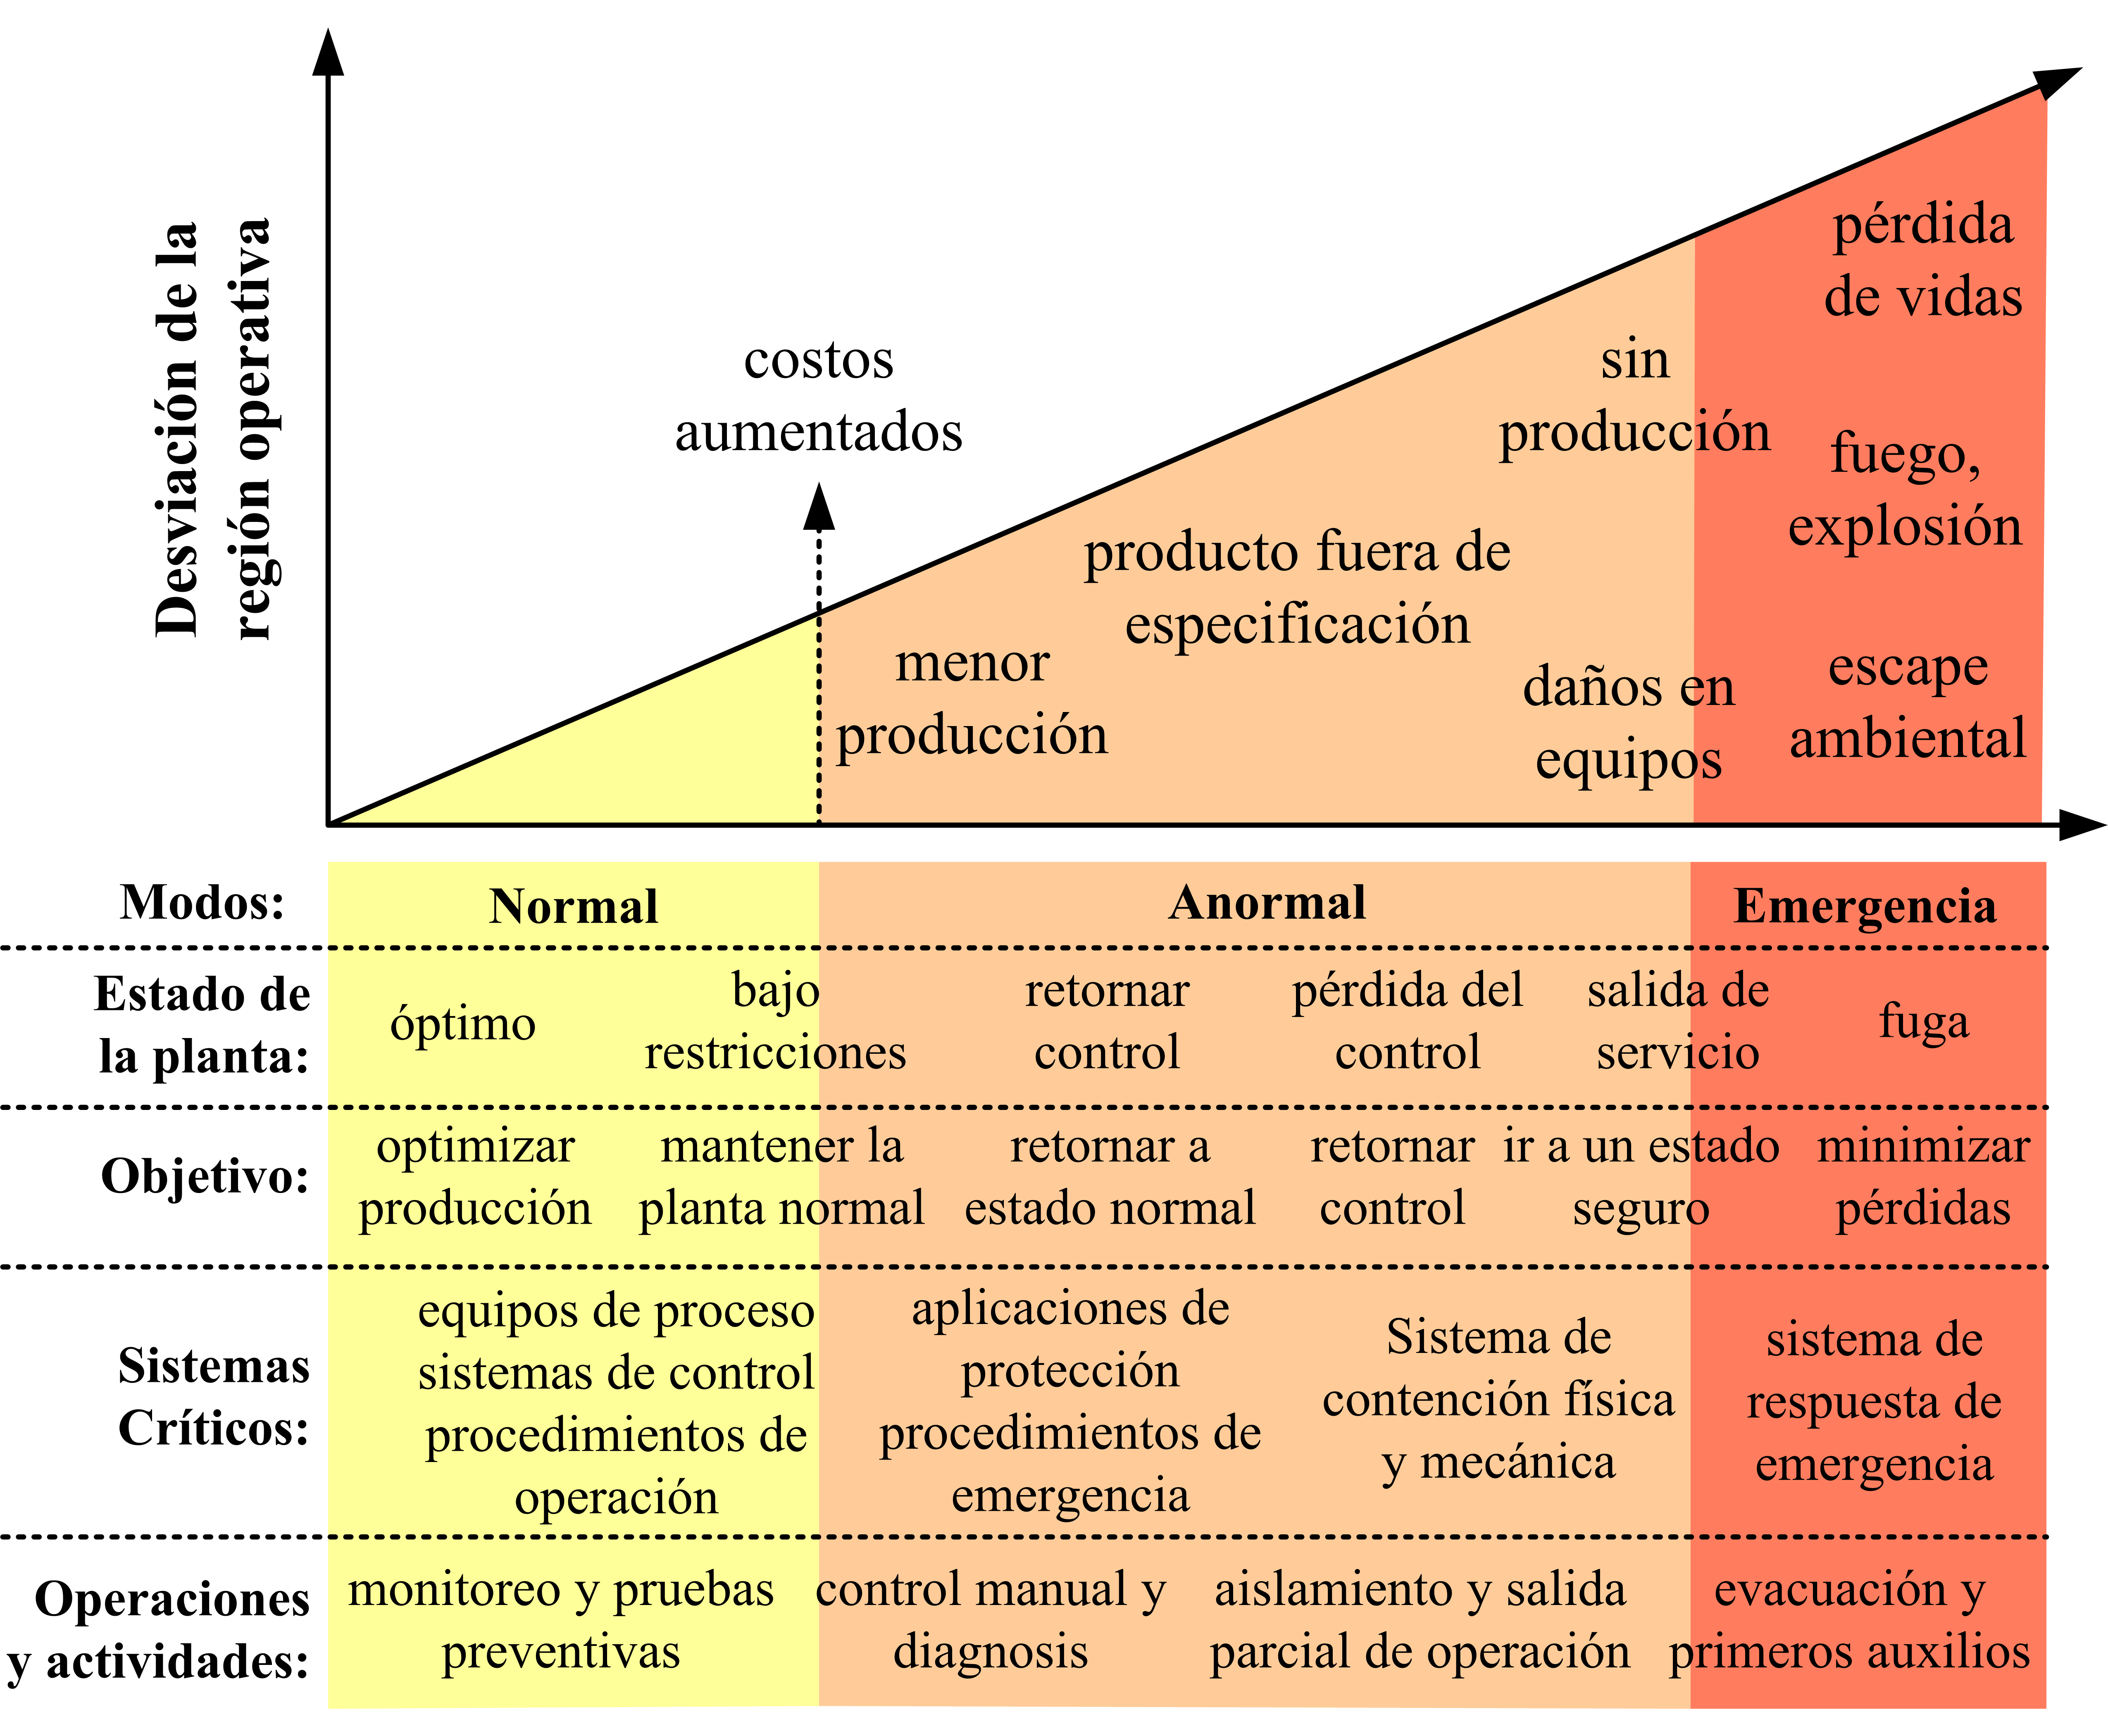
\includegraphics[width=15cm,height=13cm]{Ch0/f0_3}\\
  \caption{Anatom{\'\i}a de un incidente catastr{\'o}fico (\cite{ASM}\textcolor{myblue}{\circledR})}\label{f0_3}
\end{figure}
%------------------------------------------------------------------------------------------

La figura muestra la evoluci{\'o}n de una SA desde un trastorno de operaci{\'o}n hasta un desastre catastr{\'o}fico
involucrando destrucci{\'o}n y da{\~n}os a la planta y/o la comunidad que la rodea. En el centro de la figura
(sistemas cr{\'\i}ticos), se ilustra la progresi{\'o}n de una SA y la interacci{\'o}n con condiciones de fallas y
problemas ocultos en diferentes sistemas de la planta. Estos sistemas est{\'a}n dise{\~n}ados para salvaguardar la
integridad de la planta ante eventos catastr{\'o}ficos. El rol del personal de planta tambi{\'e}n puede apreciarse
de la figura anterior para prevenir trastornos en la operaci{\'o}n. Cuando se presenta una p{\'e}rdida de control el
personal de planta debe intervenir para minimizar el impacto del incidente.

Las actividades de operaci{\'o}n son realizadas por equipos de operaciones que comprenden: operadores de
consola, operadores principales, supervisores y operadores de campo. Esto tambi{\'e}n incluir{\'\i}a la coordinaci{\'o}n
entre los equipos responsables de las operaciones de diversas {\'a}reas dentro de la planta. Las actividades de
ayuda t{\'e}cnica son realizadas por personal t{\'\i}pico que abarca ingenieros y t{\'e}cnicos en las siguientes {\'a}reas de
proceso: instrumentaci{\'o}n, mec{\'a}nica, seguridad, desarrollo y sistemas de control. Aunque, el papel de los
individuos var{\'\i}a de situaci{\'o}n en situaci{\'o}n, el grado con el cual el personal de ayuda t{\'e}cnica se involucra
depende de la velocidad a la cual el problema se desarrolla. Desafortunadamente, el operador de consola
generalmente es el {\'u}nico habilitado a responder debido a la velocidad con que se desarrollan los eventos
anormales. La capacidad de ayuda en tiempo real del operador de consola depender{\'a} de la integraci{\'o}n y
rapidez de los sistemas de comunicaci{\'o}n.

\subsection{Impacto}
La larga historia de desastres (no debidos a causas naturales) de las plantas petroqu{\'\i}micas en Estados
Unidos fue de 1.6 billones de d{\'o}lares en 1989. En promedio, una planta petroqu{\'\i}mica tendr{\'a} un incidente
considerable cada tres a{\~n}os. Actualmente y basados en datos recogidos por compa{\~n}{\'\i}as de seguros se estima que
las p{\'e}rdidas de producci{\'o}n debido a accidentes podr{\'\i}a ser al menos de 10 billones de d{\'o}lares anualmente en
los Estados Unidos. Los costos asociados a reparaciones y/o reemplazo de equipos, multas ambientales,
compensaciones por p{\'e}rdidas humanas, investigaci{\'o}n, pleitos, etc., representan otros 10 billones
adicionales.

La mayor{\'\i}a de las situaciones anormales no resultan en explosiones pero son de todas formas situaciones que
generan costos por baja calidad del producto, retrasos, da{\~n}os de equipos, etc.. De los an{\'a}lisis de procesos
realizados en las compa{\~n}{\'\i}as miembro del consorcio de manejo de situaciones anormales resulta que entre un
3\% y un 8\% de la capacidad de la planta se pierde debido a eventos inesperados.

\section{Monitoreo de procesos}
Durante los {\'u}ltimos 30 a{\~n}os, las industrias qu{\'\i}micas y petroqu{\'\i}micas han realizado esfuerzos enormes para
reducir costos e incrementar la eficiencia de los procesos. La re-ingenier{\'\i}a, las nuevas tecnolog{\'\i}as de
sensores y los nuevos sistemas de control han contribuido a llevar a acabo este incremento de eficiencia.
Por otro lado, el escenario resultante son procesos con unidades sumamente conectadas entre si, con
complejas pol{\'\i}ticas de control, con un gran n{\'u}mero de elementos intervinientes y con un grado de robustez
relativo.

En este contexto, los operadores de proceso son quienes atienden las situaciones anormales. Generalmente,
para dar aviso de variables con valores anormales se encienden alarmas de control cl{\'a}sicas (por ejemplo,
alarmas de alto nivel o alta presi{\'o}n). Sin embargo, la complejidad de los procesos modernos hace dif{\'\i}cil la
predicci{\'o}n de eventos anormales. Las alarmas de control cl{\'a}sicas no suministran informaci{\'o}n de las causas
ra{\'\i}z de la falla, solo informan respecto de una desviaci{\'o}n particular.

El alto grado de acoplamiento de los procesos, causa que una desviaci{\'o}n pueda propagarse (r{\'a}pidamente) por
numerosos equipos haciendo dif{\'\i}cil y a veces imposible que los operarios del proceso detecten, clasifiquen y
compensen dichos eventos anormales. Adem{\'a}s, una interacci{\'o}n severa en los procesos incrementa la posibilidad
que una acci{\'o}n de control, que tiende a rechazar alg{\'u}n efecto provocado por perturbaciones en una unidad
determinada, afecte otras unidades de la planta de forma dr{\'a}stica.

Los directores y operadores de planta est{\'a}n abocados a conocer c{\'o}mo operar la planta de modo seguro y {\'o}ptimo
desde el punto de vista econ{\'o}mico. A menudo, la producci{\'o}n no se ve afectada por una disminuci{\'o}n en el
rendimeinto, pero s{\'\i} cuando una falla es realmente importante. En tales situaciones, se  generan costos
econ{\'o}micos considerables ya sea por la salida de operaci{\'o}n del proceso, da{\~n}os en los equipos, contaminaci{\'o}n
ambiental, etc.

Quiz{\'a}s el accidente qu{\'\i}mico m{\'a}s grande tom{\'o} lugar en Bhopal, India en 1984, cuando una planta de pesticida
(un subsidiario de Dow Chemical Company) accidentalmente dejo escapar gas t{\'o}xico. Mas de 3000 ciudadanos
murieron y entre de 200000 y 600000 sufrieron da{\~n}os. Este incidente provoc{\'o} alrededor de 4.1 billones de
euros de da{\~n}os econ{\'o}micos. El accidente en Bhopal fue el resultado de una combinaci{\'o}n de errores como
legales, tecnol{\'o}gicos, de organizaci{\'o}n y humanos. A continuaci{\'o}n se detallan algunos de los defectos
encontrados en la planta (\cite{Me:05,CEFIC}):
\begin{itemize}
    \item[*] El depurador de gas t{\'o}xico, dise{\~n}ado para neutralizar cualquier escape, estaba fuera de
    servicio para mantenimiento. Las investigaciones luego del desastre revelan que a{\'u}n funcionando este
    depurador pod{\'\i}a manejar s{\'o}lo un cuarto de la presi{\'o}n que alcanz{\'o} en el accidente.
    \item[*] La torre de quemado, dise{\~n}ada para quemar cualquier escape del depurador tambi{\'e}n estaba fuera
    de servicio. Adem{\'a}s tambi{\'e}n estaba mal dise{\~n}ada, s{\'o}lo pod{\'\i}a manejar un cuarto del volumen del gas
    escapado.
    \item[*] La cortina de agua. para neutralizar cualquier gas remanente, fue demasiado corta para alcanzar
    lo alto de la torre de quemado, de donde el gas fue esparcido.
    \item[*] La unidad de refrigeraci{\'o}n, que mantiene el gas a bajas temperaturas, estuvo fuera de servicio
    por alg{\'u}n tiempo.
    \item[*] El tanque de almacenamiento de gas fue llenado superando su capacidad.
    \item[*] Elementos de medici{\'o}n de temperatura y presi{\'o}n, en diferentes unidades del proceso, eran tan
    poco confiables que los operarios ignoraron signos tempranos del problema.
    \item[*] La carencia de un efectivo sistema de alarmas.
\end{itemize}

Afortunadamente, la mayor{\'\i}a de los incidentes no son tan dr{\'a}sticos. Pero de todas formas generan un
importante costo econ{\'o}mico por da{\~n}os de diferentes formas. En la {\'u}ltima d{\'e}cada, el inter{\'e}s en sistemas de
monitoreo (SM) ha aumentado siguiendo la demanda de mejor direcci{\'o}n de plantas de acuerdo con restricciones
econ{\'o}micas y ambientales, resultando en una disminuci{\'o}n de los accidentes.

Los principales objetivos de un SM son minimizar los riesgos e incrementar la calidad de la producci{\'o}n. Un
SM debe trabajar en tiempo real, 24 horas del d{\'\i}a, los 365 d{\'\i}as del a{\~n}o, detectando tantos eventos anormales
como sea posible (mucho antes que las alarmas de control) e informando de forma adecuada al operador sobre
el estado del proceso, causas ra{\'\i}z y soluciones sugeridas. Por lo tanto, pueden tomarse acciones apropiadas
en tiempo real para evitar la propagaci{\'o}n de la falla o su eventual compensaci{\'o}n y tender a reducir lo
m{\'a}ximo posible las consecuencias de dicho evento anormal.
